\documentclass[11pt,pdf,hyperref={unicode}]{beamer}
\usepackage[english,russian]{babel}
\usepackage{sidecap}
\usepackage{geometry}

% подключаем кириллицу 
\usepackage[T2A]{fontenc}
\usepackage[utf8]{inputenc}

\usepackage{wrapfig}
\usepackage[makeroom]{cancel}
\usepackage{braket}
\usepackage{amsmath}
\usepackage{graphicx}
\usepackage{amssymb}

\usepackage{bookmark}
% \usepackage{etoolbox}

% отключить клавиши навигации
% \setbeamertemplate{navigation symbols}{}

\usetheme{Malmoe}
\usefonttheme[onlymath]{serif}
\usecolortheme{seahorse}

\title[Выделение сообществ в графах \hspace*{1cm} SCVRT2015]{Разработка и реализация моделей и алгоритмов выделения сообществ в графах взаимодействующих объектов}
\author[C. Шилин]{Сергей Шилин \vspace{-0.6cm}}
\date[SCVRT2015]{Международная конференция SCVRT2015 \break 24-27 ноября 2015 г. }
\titlegraphic{
\includegraphics[width=2cm]{images/FTI-logo.jpg}\hspace*{4.75cm}~%
   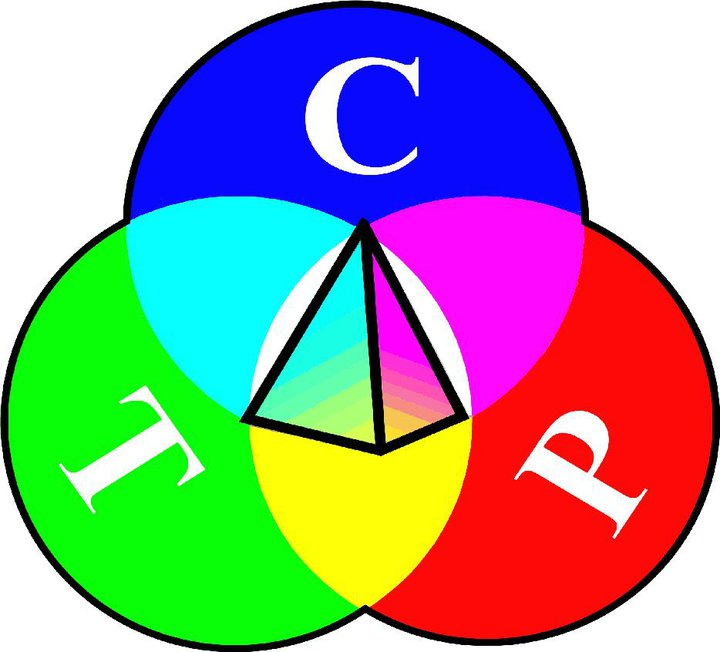
\includegraphics[width=2cm]{images/IFTI-FTI-logotip.jpg}\vspace{1.5cm}
}

% \makeatletter
% \apptocmd{\beamer@@frametitle}{\bookmark[page=\the\c@page,level=4]{#1}}%
% {\message{** patching of \string\beamer@@frametitle succeeded **}}%
% {\message{** patching of \string\beamer@@frametitle failed **}}%
% \makeatother

\setbeamertemplate{section in toc}[sections numbered]
\setbeamertemplate{subsection in toc}[ball unnumbered]
\setbeamertemplate{itemize items}[ball]
\setbeamertemplate{enumerate items}[ball]
\setbeamertemplate{caption}[numbered]
\addtobeamertemplate{navigation symbols}{}{%
    \usebeamerfont{footline}%
    \usebeamercolor[fg]{footline}%
    \hspace{1em}%
    \insertframenumber/\inserttotalframenumber
}


\begin{document}

% титульный слайд
\frame{\titlepage}
\begin{frame}{Содержание}
	\tableofcontents
\end{frame}

\section{Введение} % (fold)
\label{sec:intro}

	\subsection{Социальный граф} % (fold)
	\label{sub:socgraph}
		\begin{frame}{Введение: Социальный граф} 
			\begin{enumerate}
				\item Одна большая общая компонента связности
				\pause \item Распределение на степенях вершин
				\pause \item Среднее расстояние
				\pause \item Коэффициент кластеризации
				\pause \item Структура сообществ
			\end{enumerate}
		\end{frame}

	\subsection{Сообщество} % (fold)
	\label{sub:community}
		\begin{frame}{Введение: Сообщество}
			\begin{itemize}
				\item Формально : структура графа образована сообществами, если он отличается от случайного графа.
				\pause \item С содержательной точки зрения -- это группа вершин сети, участники которой связаны друг с другом значительно теснее, чем с остальными вершинами сети.
			\end{itemize}
		\end{frame}

	\subsection{Проблема} % (fold)
	\label{sub:problem}
		\begin{frame}{Введение: Проблема}
			\begin{itemize}
				\item Проблема выделения сообществ есть задача анализа графов.
				\pause \item Существует множество алгоритмов с использованием методов из различных дисциплин. Не все алгоритмы надёжны и могут быть применены на практике.
				\pause \item Не понятно, как хранить и анализировать графы очень больших размеров.
				\pause \item \textbf{Задача} -- Для конкретной задачи разработать алгоритм выделения сообществ, который покажет хорошие результаты для конкретной задачи в сравнении с существующими методами.
			\end{itemize}
		\end{frame}

		\begin{frame}{Пример: кластеризация веб-доменов}
			Есть данные о посещениях пользователями различных доменов, есть граф, где в качестве узлов выступают домены, а в качестве рёбер -- аффинити между доменами. \newline
			\newline
			Аффинити между доменами $x$ и $y$ -- это выборочная оценка того, насколько события «посещение юзером $u$ домена $x$» и «посещение юзером $u$ домена $y$» близки к независимости. 
		\end{frame}

		\begin{frame}{Пример: кластеризация веб-доменов}
			\begin{figure}[h]
				\centering
				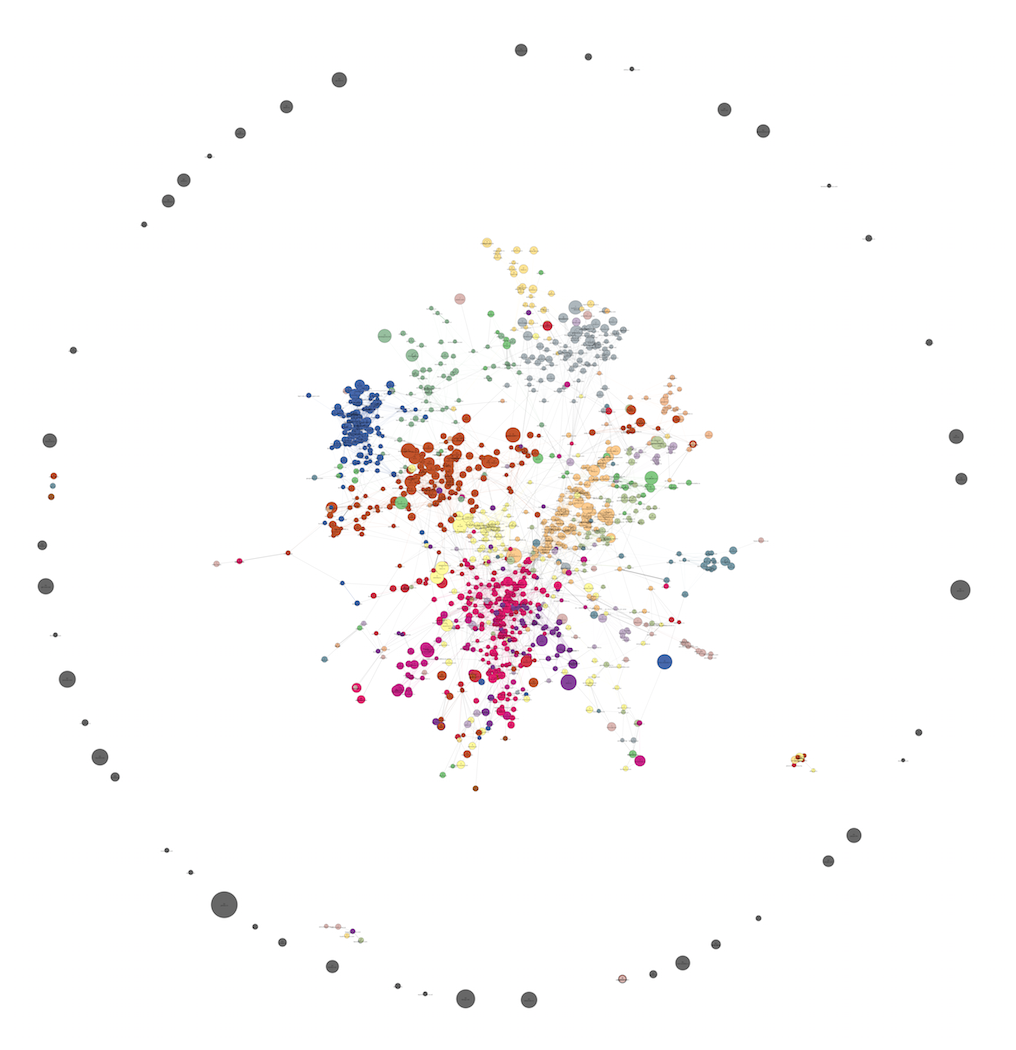
\includegraphics[width=5.7cm]{images/graph-domains.png}
				\caption{Кластеризация графа для 1285 доменов}
				\label{fig:domains}
			\end{figure}
		\end{frame}

% section intro (end)

\section{Выделения сообществ} % (fold)
\label{sec:clustering}

	\subsection{Критерии качества} % (fold)
	\label{sub:quality}
		\begin{frame}{Критерии качества} 
			После того как отработал алгоритм выделения сообществ, необходимо оценить качество получившегося результата.
			\begin{itemize}
				\item Модулярность
				$$
				Q = \frac{1}{2m} \displaystyle\sum_{i,j}\left(A_{ij} - \frac{d_i d_j}{2m}\right)\delta(C_i,C_j)
				$$
				\pause \item Редакторское расстояние для разбиений (split-join distance)
				\pause \item Нормализованная взаимная информация
			\end{itemize}
		\end{frame}

	\subsection{Алгоритмы: igraph} % (fold)
	\label{sub:algos}
		\begin{frame}{Алгоритмы: igraph}
			\begin{itemize}
				\item \textbf{Betweenness} коэффициент «центральности по посредничеству» (Betweenness)
				\pause \item \textbf{Fastgreedy} жадная оптимизация функции модулярности
				\pause \item \textbf{Multilevel} многоуровневая оптимизация функции модулярности с эвристикой
				\pause \item \textbf{LabelPropogation} присвоение меток к каждой вершине
				\pause \item \textbf{Walktrap} короткие случайные блуждания не приводят к выходу из текущего сообщества
				\pause \item \textbf{Infomap} случайное блуждание, основанное на понятии информационных потоков в сетях, кодирования и сжатия информации
				\pause \item \textbf{Eigenvector} собственных векторах матрицы модулярности, которая получается из матрицы смежности
			\end{itemize}
		\end{frame}

	\subsection{Тестирование алгоритмов} % (fold)
	\label{sub:testing}
		\begin{frame}{Тестирование алгоритмов}
			\begin{itemize}
				\item Моделирование данных
				\begin{enumerate}
					\item Генерация графа
					\item Зашумление графа
				\end{enumerate}
				\pause \item Реальные данные
			\end{itemize}
		\end{frame}

% section clustering (end)

\section{Вывод} % (fold)
\label{sec:outro}

	\subsection{Актуальность задачи} % (fold)
	\label{sub:actual}
		\begin{frame}{Актуальность задачи}
			\begin{itemize}
				\item Распознавание структуры, скрытой в реальных социальных сетях, является ключевой задачей, решение которой необходимо для понимания организации сложных сетей.
				\pause \item Кластеризация элементов сложных сетей позволяет анализировать их на более высоком уровне, что в разы проще.
			\end{itemize}
		\end{frame}

% section outro (end)
	


\end{document}